\usetikzlibrary{arrows.meta,calc}
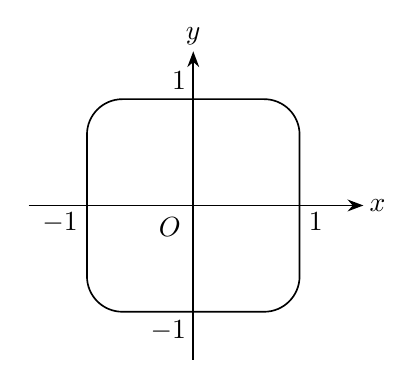
\begin{tikzpicture}[x=1.35cm,y=1.35cm,line width=.6pt,font=\normalsize,>=Stealth]
\coordinate (O) at (0,0);
\draw[->] (-1.55,0)--(1.6,0) node[right,inner sep=0pt,xshift=2pt] {$x$};
\draw[->] (0,-1.45)--(0,1.45) node[above,inner sep=0pt,yshift=2pt] {$y$};
\draw[rounded corners=0.45cm] (-1,-1)--(1,-1)--(1,1)--(-1,1)--cycle;
\node[anchor=north east,inner sep=0pt] at (-1.08,-0.06) {$-1$};
\node[anchor=north west,inner sep=0pt] at (1.08,-0.06) {$1$};
\node[anchor=south east,inner sep=0pt] at (-0.06,1.08) {$1$};
\node[anchor=north east,inner sep=0pt] at (-0.06,-1.08) {$-1$};
\node[anchor=center,inner sep=0pt] at (-0.22,-0.20) {$O$};
\end{tikzpicture}
